\documentclass[dvipdfmx]{report} % 文章の形式を設定
\usepackage[margin=2.5cm]{geometry} % 書式の空白を設定
\usepackage[utf8]{inputenc} % 文字コードをUTF-8に設定
\usepackage{hyperref} % 目次にリンクを付けるため
\usepackage{lipsum} % ダミーテキスト用
\usepackage{tcolorbox} % 枠を利用するため
\usepackage{amsmath} % 数式の記述を行うため
\usepackage{bm} % ベクトルを太字で表示するため
\usepackage{graphicx} % 画像を表示するため
\usepackage{float} % 画像正しい位置で表示するため
\usepackage{tensor} % テンソルを記載するため
\usepackage{multicol} % 複数段落を作成するため
\usepackage{tikz} % 図を作成するため
\usepackage{amssymb} % 特殊文字を表示するため
\usepackage{enumerate} % リストを作成するため


\title{勉強したことのまとめ}
\author{大豆生田 幹}
\date{}

\begin{document}

\maketitle % タイトルの作成
\tableofcontents % 目次の作成

% =================================
% =================================
% =================================
% =================================
% =================================
% 一般相対論
% =================================
% =================================
% =================================
% =================================
% =================================
\chapter{07/08/2024}

\section{光の測地線方程式}
粒子の場を表す方程式である、クラインゴルドン方程式
\[ \left( \frac{1}{c^2}\frac{\partial^2}{\partial t^2} - \nabla^2 + \left( \frac{mc}{\hbar} \right)^2 \right) \phi(\bm{x}, t) = 0 \]
質量のない光では
\begin{equation*}
\begin{split}
	0 &= \left( \frac{1}{c^2}\frac{\partial^2}{\partial t^2} - \nabla^2 \right)\phi(\bm{x}, t)\\
	&= \square \phi(\bm{x}, t)
\end{split}
\end{equation*}
これを一般の時空に拡張すると
\[ g^{ij} \nabla_i \nabla_j \phi = 0 \]
ここで、\[ \phi = Ce^{i\frac{s}{\epsilon}} \] と書くと
\begin{equation*}
\begin{split}
	\nabla_j \phi &= \nabla \left( Ce^{\frac{is}{\epsilon}} \right)\\
	&= \left( \nabla_j C \right) e^{\frac{is}{\epsilon}} + \frac{iC}{\epsilon} e^{\frac{is}{\epsilon}} \left( \nabla_j S \right)\\
	\nabla_i \nabla_j \phi &= \nabla_i \left(  \left( \nabla_j C \right) e^{\frac{is}{\epsilon}} + \frac{iC}{\epsilon} e^{\frac{is}{\epsilon}} \left( \nabla_j S \right) \right)\\
	&= \left( \nabla_i \nabla_j C \right) e^{\frac{is}{\epsilon}} + \left( \nabla_i S \right) \left( \nabla_j C \right) \frac{2i}{\epsilon} e^{\frac{is}{\epsilon}} + \left( \nabla_i \nabla_j S \right) \frac{iC}{\epsilon} e^{\frac{is}{\epsilon}} -  \left( \nabla_i S \right) \left( \nabla_j S \right) \frac{1}{\epsilon^2} e^{\frac{2is}{\epsilon}}\\
	g^{ij} \nabla_i \nabla_j \phi &= g^{ij}\left( \nabla_i \nabla_j C \right) e^{\frac{is}{\epsilon}} + g^{ij}\left( \nabla_i S \right) \left( \nabla_j C \right) \frac{2i}{\epsilon} e^{\frac{is}{\epsilon}} + g^{ij}\left( \nabla_i \nabla_j S \right) \frac{iC}{\epsilon} e^{\frac{is}{\epsilon}} -  g^{ij}\left( \nabla_i S \right) \left( \nabla_j S \right) \frac{1}{\epsilon^2} e^{\frac{2is}{\epsilon}}\\
	&= \left( \square C \right) e^{\frac{is}{\epsilon}} + \left( \nabla_i S \right) \left( \nabla^i C \right) \frac{2i}{\epsilon} e^{\frac{is}{\epsilon}} + \left( \square S \right) \frac{iC}{\epsilon} e^{\frac{is}{\epsilon}} -  \left( \nabla_i S \right) \left( \nabla^i S \right) \frac{1}{\epsilon^2} e^{\frac{2is}{\epsilon}}
\end{split}
\end{equation*}
\begin{equation}
\left\{ \,
\begin{aligned}
	O(\epsilon^{-2}) &: \left( \nabla_i S \right) \left( \nabla^i S \right) = 0\\
	O(\epsilon^{-1}) &: 2 \left( \nabla_i S \right) \left( \nabla^i C \right) + C \left( \square S \right) = 0\\
	O(0) &: \square C = 0
\end{aligned}
\right.
\end{equation}
ここで、\[ \left( \nabla_i S \right) \left( \nabla^i S \right) = 0 \]は光の測地線方程式を表している。
\[ \nabla_i S  =  k_i \]とおけば
\begin{equation*}
\begin{split}
	0 &= \left( \nabla_i S \right) \left( \nabla^i S \right)\\
	&= k_i k^i\\
	&= \nabla_j (k_i k^i)\\
	&= \nabla_j (k_i g^{ij} k_l)\\
	&= g^{il} (\nabla_j k_l)k_i + g^{il} (\nabla_j k_i)k_l\\
	&= 2(\nabla_j k_i)k^i\\
	&= 2 g^{lj} (\nabla_j \nabla_i S)k^i\\
	&= 2 (\nabla_i g^{lj}  k_j)k^i\\
	&= 2 (\nabla_i k^l)k^i\\
	&= 2\left( \frac{\partial}{\partial x^i} \left( \frac{dx^l}{d\lambda} \right) + \tensor{\Gamma}{^l_{im}} \left( \frac{dx^m}{d\lambda} \right) \right) \frac{dx^i}{d\lambda}
\end{split}
\end{equation*}
\begin{tcolorbox}[title=光の測地線方程式]
\begin{eqnarray*}
	0 = \left( \frac{d^2 x^l}{d\lambda^2} \right) + \tensor{\Gamma}{^l_{im}} \left( \frac{dx^i}{d\lambda}\frac{dx^m}{d\lambda} \right)
\end{eqnarray*}
\end{tcolorbox}

\section{積分}
\begin{equation*}
\begin{split}
	\left( \frac{d\mu}{d\phi} \right)^2 &= 2MG(\mu)\\
	\frac{d\mu}{d\phi} &= - \sqrt{2MG(\mu)}\\
\end{split}
\end{equation*}

\begin{equation}
\left\{ \,
\begin{aligned}
	\mu_1 &= - \frac{Q + 2M - P}{4MP}\\
	\mu_2 &= - \frac{1}{P}\\
	\mu_3 &= - \frac{Q - 2M + P}{4MP}\\
\end{aligned}
\right.
\end{equation}

\begin{equation*}
\begin{split}
	\int^{\phi_\infty}_0 d\phi &= \int^{0}_{\mu_2} \frac{d\mu}{- \sqrt{2MG(\mu)}}\\
	\phi_{\infty} &= \frac{1}{\sqrt{2M}} \int^{\mu_2}_{0} d\mu \left( (\mu - \mu_1)(\mu - \mu_2)(\mu - \mu_3) \right)^{- \frac{1}{2}}\\
\end{split}
\end{equation*}
ここで、
\begin{equation*}
\begin{split}
	\chi &= \sqrt{\mu - \mu_1}\\
	d\chi &= \frac{1}{2}(\mu - \mu_1)^{- \frac{1}{2}} d\mu
\end{split}
\end{equation*}
とおくと
\begin{equation*}
\begin{split}
	\phi_{\infty} &= \frac{1}{\sqrt{2M}} \int^{\sqrt{\mu_2 - \mu_1}}_{\sqrt{-\mu_1}} \frac{ 2\chi d\chi }{\sqrt{ \chi^2(\chi^2 + \mu_1 - \mu_2)(\chi^2 + \mu - \mu_3) }}\\
\end{split}
\end{equation*}
ここで、
\begin{equation*}
\begin{split}
	\chi &= \sqrt{\mu_2 - \mu_1}\eta\\
	d\chi &= \sqrt{\mu_2 - \mu_1}d\eta
\end{split}
\end{equation*}
とおくと
\begin{equation*}
\begin{split}
	\phi_{\infty} &= \frac{2}{\sqrt{2M}} \int^{1}_{\sqrt{\frac{\mu_1}{\mu_1 - \mu_2}}} \frac{ \sqrt{\mu_2 - \mu_1} d\eta }{\sqrt{ -(\mu_2 - \mu_1)(1 - \eta^2)((\mu_2 - \mu_1)\eta^2 - \mu_1 + \mu_3) }}\\
\end{split}
\end{equation*}
ここで、
\begin{equation*}
\begin{split}
	\eta &= \sin x\\
	d\eta &= dx \cos x
\end{split}
\end{equation*}
とおくと
\begin{equation*}
\begin{split}
	\phi_{\infty} &= \frac{2}{\sqrt{2M}} \int^{\frac{\pi}{2}}_{\sin^{-1}\sqrt{\frac{\mu_1}{\mu_1 - \mu_2}}} \frac{ \cos x dx }{\sqrt{\cos^2 x} \sqrt{ -(\mu_2 - \mu_1)\sin^2 x((\mu_2 - \mu_1)\eta^2 - \mu_1 + \mu_3) }}\\
	&= \frac{2}{\sqrt{2M}} \int^{\frac{\pi}{2}}_{\sin^{-1}\sqrt{\frac{\mu_1}{\mu_1 - \mu_2}}} \frac{ dx }{ \sqrt{\mu_3 - \mu_1} \sqrt{ - \frac{\mu_2 - \mu_1}{\mu_3 - \mu_1}\sin^2 x + 1) }}\\
\end{split}
\end{equation*}

\begin{equation}
\left\{ \,
\begin{aligned}
	\mu_3 - \mu_1 &= \frac{Q}{2MP}\\
	\mu_2 - \mu_1 &= \frac{Q + 6M - P}{4MP}\\
\end{aligned}
\right.
\end{equation}

\begin{equation}
\left\{ \,
\begin{aligned}
	\frac{\mu_2 - \mu_1}{\mu_3 - \mu_1} &= \frac{Q + 6M - P}{2Q}\\
	\frac{\mu_1}{\mu_1 - \mu_2} &= \frac{Q + 2M - P}{Q + 6M - P}\\
\end{aligned}
\right.
\end{equation}

\begin{equation*}
\begin{split}
	\phi_{\infty} &= \frac{2}{\sqrt{2M}} \int^{\frac{\pi}{2}}_{\sin^{-1}\sqrt{\frac{Q + 2M - P}{Q + 6M - P}}} \frac{ dx }{\sqrt{\frac{Q}{2MP}} \sqrt{ 1 - \frac{Q + 6M - P}{2Q} \sin^2 x }}\\
\end{split}
\end{equation*}
ここで、
\begin{equation*}
\begin{split}
	\kappa &= \sqrt{ \frac{Q+6M-P}{2Q} }\\
	\zeta &= \sin^{-1} \sqrt{\frac{Q+2M-P}{Q+6M-P}}
\end{split}
\end{equation*}
さらに
\begin{equation*}
\begin{split}
	K(\kappa) &= \int^{\frac{\pi}{2}}_{0} \frac{ dx }{\sqrt{ 1 - \kappa^2 \sin^2 x }}\\
	F(\zeta, \kappa) &= \int^{\zeta}_{0} \frac{ dx }{\sqrt{ 1 - \kappa^2 \sin^2 x }}\\
\end{split}
\end{equation*}

とおくと
\begin{tcolorbox}[title=$\phi_{\infty}$についての式]
\begin{eqnarray*}
\begin{split}
	\phi_{\infty} &= 2\sqrt{ \frac{P}{Q} } \int^{\frac{\pi}{2}}_{\zeta} \frac{ dx }{\sqrt{ 1 - \kappa^2 \sin^2 x }}\\
	&= 2\sqrt{ \frac{P}{Q} }\left( K(\kappa) - F(\zeta, \kappa) \right)
\end{split}
\end{eqnarray*}
\end{tcolorbox}

\chapter{28/08/2024}

\section{$P \gg M$}

\begin{equation*}
\left\{ \,
\begin{aligned}
	Q &\approx P \left( 1 + 2\left( \frac{M}{P} \right) - 8\left( \frac{M}{P} \right)^2 \right)\\
	\kappa^2 &\approx 4\left( \frac{M}{P} \right)\\
	\zeta &\approx \frac{\pi}{4} - \frac{1}{2} \left( \frac{M}{P} \right)\\
\end{aligned}
\right.
\end{equation*}

以上を考慮して$\phi_{\infty}$を計算する
\begin{equation*}
\begin{split}
	\phi_{\infty} &= 2\sqrt{ \frac{P}{Q} } \int^{\frac{\pi}{2}}_{\zeta} \frac{ dx }{\sqrt{ 1 - \kappa^2 \sin^2 x }}\\
	&\approx 2\sqrt{ \frac{P}{Q} } \int^{\frac{\pi}{2}}_{\zeta} \left( 1 + \frac{1}{2}\kappa^2 \sin^2 x \right) dx\\
	&= 2\sqrt{ \frac{P}{Q} } \int^{\frac{\pi}{2}}_{\zeta} \left( 1 + \frac{1}{2}\kappa^2 - \frac{1}{4}\kappa^2 \cos 2x \right) dx\\
	&\approx 2\left( 1 - \frac{M}{P} \right)\int^{\frac{\pi}{2}}_{\frac{\pi}{4} - \frac{M}{2P}} \left( 1 + 2\frac{M}{P} - \frac{M}{P} \cos 2x \right)dx\\
	&= 2\left( 1 - \frac{M}{P} \right) \left[ x + \frac{M}{P}x - \frac{M}{2P} \sin 2x\right]^{\frac{\pi}{2}}_{\frac{\pi}{4} - \frac{M}{2P}}\\
	&= \frac{\pi}{2} + \frac{2M}{P}
\end{split}
\end{equation*}

\section{$P \approx 3M( 1 + \epsilon )$}

\begin{equation*}
\left\{ \,
\begin{aligned}
	Q &\approx 3M + 5M\epsilon\\
	\kappa &\approx 1 - \frac{2}{3}\epsilon\\
	\zeta &\approx \sin^{-1} \sqrt{ \frac{1}{3} } + \frac{\sqrt{3}}{9\cos \left( \sin^{-1} \sqrt{ \frac{1}{3} } \right) }\epsilon\\
	\sqrt{ \frac{P}{Q} } &\approx 1 - \frac{1}{3}\epsilon\\
	\sqrt{ 1 - \kappa^2 } &\approx \sqrt{ \frac{4}{3} \epsilon }\\
	b &\approx b_c \left( 1 + \frac{3}{2}\epsilon^2 \right)\\
\end{aligned}
\right.
\end{equation*}

\begin{tcolorbox}[title=$ \kappa \approx 1 $での公式]
\begin{eqnarray*}
\begin{split}
	K(\kappa) &= \ln \frac{4}{\kappa'} + \left( \frac{1}{2} \right)^2 \left( \ln \frac{4}{\kappa'} - \frac{2}{1 \cdot 2} \right) \kappa'^2 + \left( \frac{1 \cdot 3}{2 \cdot 4} \right)^2 \left( \ln \frac{4}{\kappa'} - \frac{2}{1 \cdot 2} - \frac{2}{3 \cdot 4} \right) \kappa'^4 + ... \\
	F(\zeta, \kappa) &= \frac{2}{\pi} \bm{K'} \ln \tan \left( \frac{\zeta}{2} + \frac{\pi}{4} \right) - \frac{\tan \zeta}{\cos \zeta} \left( a'_0 - \frac{2}{3}a'_1\tan^2 \zeta + ... \right)
\end{split}
\end{eqnarray*}
\begin{equation*}
\left\{ \,
\begin{aligned}
	a'_0 &= \frac{2}{\pi}\bm{K'} - 1\\
	a'_n &= a'_{n-1} - \left[ \frac{(2n-1)!!}{2^{n}n!} \right]^2 \kappa'^{2n}
\end{aligned}
\right.
\end{equation*}
\begin{equation*}
\begin{split}
	\bm{K'} &= \frac{\pi}{2} \left( 1 + \left( \frac{1}{2} \right)^2 \kappa'^2 + ... \right)\\
	\kappa' &= \sqrt{1-\kappa^2}
\end{split}
\end{equation*}
\end{tcolorbox}

以上を考慮して$b$を計算する

\begin{eqnarray*}
\begin{split}
	K(\kappa) &\approx \ln \frac{4}{\kappa'}\\
	F(\zeta, \kappa) &\approx \ln \tan \left( \frac{\zeta}{2} + \frac{\pi}{4} \right)\\
\end{split}
\end{eqnarray*}

\begin{eqnarray*}
\begin{split}
	\phi_{\infty} &= 2\sqrt{ \frac{P}{Q} }\left( K(\kappa) - F(\zeta, \kappa) \right)\\
	&\approx 2\left( 1 - \frac{\epsilon}{3} \right) \left( \ln \frac{4}{\kappa'} - \ln \tan \left( \frac{\zeta}{2} + \frac{\pi}{4} \right) \right)\\
	&= \left( 1 - \frac{\epsilon}{3} \right) \ln \left( \frac{ \frac{12}{\epsilon} }{ \tan^2 \left( \frac{\sin^{-1} \sqrt{\frac{1}{3}}}{2} + \frac{\pi}{4} \right) } \right)\\
	&\approx \ln \left( \frac{ 12 }{ \tan^2 \left( \frac{\sin^{-1} \sqrt{\frac{1}{3}}}{2} + \frac{\pi}{4} \right) \epsilon } \right) = \ln \frac{\alpha}{\epsilon}\\
\end{split}
\end{eqnarray*}
ここで、
\[ \phi_\infty = \frac{1}{2}\pi + \frac{1}{2}\mu \]
より、
\begin{eqnarray*}
\begin{split}
	\frac{\alpha}{\epsilon} &= \exp \left( \frac{\pi}{2} + \frac{\mu}{2} \right)\\
	\epsilon &= \frac{ \alpha }{ \exp \left( \frac{\pi}{2} + \frac{\mu}{2} \right) }
\end{split}
\end{eqnarray*}
したがって
\begin{eqnarray*}
\begin{split}
	b &\approx b_c \left( 1 + \frac{3}{2}\epsilon^2 \right)\\
	&= b_c \left( 1 + \frac{3}{2} \left( \frac{ \alpha }{ \exp \left( \frac{\pi}{2} + \frac{\mu}{2} \right) } \right)^2 \right)\\
	&= b_c \left( 1 + \frac{3}{2} \alpha^2 e^{-\mu} e^{-\pi} \right)\\
	&\approx 5.19615M + 3.48228Me^{-\mu}\\
\end{split}
\end{eqnarray*}

\chapter{23/09/2024}
\section{3次式の解}

\[ b^2 = \frac{P^3}{P-2M} \]
この$P$を$b$について解きたい
\begin{equation*}
\left\{ \,
\begin{aligned}
	P &= yM\\
	b &= xM\\
\end{aligned}
\right.
\end{equation*}
と置き、$y$を$x$について解く問題を考える。

\begin{equation*}
\begin{split}
	0 &= P^3 - Pb^2 + 2Mb^2\\
	0 &= y^3M^3 - yx^2M^3 + 2x^2M^3\\
	0 &= y^3 - yx^2 + 2x^2\\
\end{split}
\end{equation*}
\[ y = u + v \]
とおくと

\begin{equation*}
\begin{split}
	0 &= ( u + v )^3 - ( u + v ) x^2 + 2 x^2\\
	0 &= (u^3 + v^3 + 2 x^2) + ( 3uv - x^2 )( u + v ) \\
\end{split}
\end{equation*}
\[ u + v \neq 0 \] と仮定すると

\begin{equation}
\left\{ \,
\begin{aligned}
	u^3 + v^3 + 2 x^2 &= 0\\
	3uv - x^2 &= 0\\
\end{aligned}
\right.
\end{equation}
以上より、片方の符号を採用すると

\begin{equation}
\left\{ \,
\begin{aligned}
	u^3 &= - x^2 + x^2 \sqrt{ 1 - \left( \frac{ x }{ 3\sqrt{3} } \right)^2 }\\
	v^3 &= - x^2 - x^2 \sqrt{ 1 - \left( \frac{ x }{ 3\sqrt{3} } \right)^2 }
\end{aligned}
\right.
\end{equation}
ここで$(u, v)$の3乗根の主値をそれぞれ$(\alpha, \beta)$とおくと

\begin{equation*}
\begin{split}
	\alpha &= \left( - x^2 + x^2 \sqrt{ 1 - \left( \frac{ x }{ 3\sqrt{3} } \right)^2 } \right) ^{\frac{1}{3}}\\
	\beta &= \left( - x^2 - x^2 \sqrt{ 1 - \left( \frac{ x }{ 3\sqrt{3} } \right)^2 } \right) ^{\frac{1}{3}}\\
	\omega &= \exp \left(\frac{2}{3} \pi i \right)
\end{split}
\end{equation*}

\begin{enumerate}[(1)\,]
\item{$D < 0 $では$(x > 3 \sqrt{3})$}
\begin{equation*}
\begin{split}
	( u, v ) =\
		\begin{cases}
			( \alpha, \beta )\\
			( \omega\alpha, \omega^2 \beta )\\
			( \omega^2 \alpha, \omega\beta )\\
		\end{cases}
\end{split}
\end{equation*}

\item{$D = 0 $では$(x = 3 \sqrt{3})$}
\begin{equation*}
\begin{split}
	( u, v ) =\
		\begin{cases}
			( \omega\alpha, \omega\beta )\\
			( \alpha, \omega^2 \beta )\\
			( \omega^2 \alpha, \beta )\\
		\end{cases}
\end{split}
\end{equation*}

\item{$D > 0 $では$(x < 3 \sqrt{3})$}
\begin{equation*}
\begin{split}
	( u, v ) =\
		\begin{cases}
			( \omega\alpha, \omega\beta )\\
			( \alpha, \omega^2 \beta )\\
			( \omega^2 \alpha, \beta )\\
		\end{cases}
\end{split}
\end{equation*}
\end{enumerate}

% =================================
% =================================
% =================================
% =================================
% =================================
% Buchdahl
% =================================
% =================================
% =================================
% =================================
% =================================
\chapter{07/01/2025}
\section{Buchdahl時空における光の軌道}
Buchdahl時空の計量は以下のように与えられる。
\begin{equation*}
\begin{split}
	g_{ij} &= \mathrm{diag}
	\left(
		- \frac{(1 - f(r))^2}{(1 + f(r))^2},
		(1 + f(r))^4,
		r^2(1 + f(r))^4 ,
		r^2 (1 + f(r))^4 \sin ^2 \theta 
	\right)\\
	f(r) &= \frac{a}{2\sqrt{1 + k r^2}} 
\end{split}
\end{equation*}
測地線を考えるには、赤道面$ \theta = \frac{\pi}{2} $に注目すれば
\begin{equation*}
\begin{split}
	S &= \int \mathcal{L} d\tau \\
	&= \int \left(
		- \frac{(1 - f(r))^2}{(1 + f(r))^2} \dot{t}^2
		+ (1 + f(r))^4 \dot{r}^2
		+ r^2(1 + f(r))^4 \dot{\phi}^2
	\right) d\tau
\end{split}
\end{equation*}
この変分を計算すれば良い。$ \mathcal{L} $は$t, \phi$をあらわには含まないので、オイラーラグランジュ方程式より
\begin{equation*}
\begin{split}
	0 &
		= - \frac{1}{2}\left( \frac{d\mathcal{L}}{d\dot{t}} \right)
		= \frac{ (1 - f(r))^2 }{(1 + f(r))^2} \dot{t}\\
	&\therefore  E = \frac{(1 - f(r))^2 }{(1 + f(r))^2} \dot{t}\\
	0 &
		= \frac{1}{2}\left( \frac{d\mathcal{L}}{d\dot{\phi}} \right)
		= r^2 (1 + f(r))^4  \dot{\phi}\\
	&\therefore  L = r^2 (1 + f(r))^4  \dot{\phi}\\
\end{split}
\end{equation*}
また、nullの条件$0 = g_{ij}\dot{x}^i\dot{x}^j$より
\begin{equation*}
\begin{split}
	0 &=
		- \frac{(1 - f(r))^2}{(1 + f(r))^2} \dot{t}^2
		+ (1 + f(r))^4 \dot{r}^2
		+ r^2(1 + f(r))^4 \dot{\phi}^2\\
	& \therefore 
		\left( \frac{E}{L} \right)^2 =
			\frac{(1 - f(r))^2}{r^4 (1 + f(r))^6} \left( \frac{dr}{d\phi} \right)^2
			+ \frac{(1 - f(r))^2}{r^2 (1 + f(r))^6}
\end{split}
\end{equation*}
ここで$u = \frac{1}{r}$、$b = \frac{L}{E}$とおくと
\[ 1 = r^4 \left( \frac{du}{dr} \right) ^2 \]より
\begin{equation*}
\begin{split}
	\left( \frac{1}{b} \right)^2 &=
		\frac{(1 - f(1/u))^2}{(1 + f(1/u))^6} \left( \frac{du}{d\phi} \right)^2
		+ \frac{u^2 (1 - f(1/u))^2}{(1 + f(1/u))^6}\\
	& \therefore \left( \frac{du}{d\phi} \right)^2 = G(u) :=
		\left( \frac{1}{b} \right)^2 \frac{(1 + f(1/u))^6}{(1 - f(1/u))^2} - u^2
\end{split}
\end{equation*}

\section{パラメータ$a$の条件}
まず、$a=0$、$k=0$は距離に依存しない時空となるので今回は考えないことする。
\subsection{$f(r)$による制約}
$ |f(r)|=1 $ではクリストッフェルスカラーが発散する。これは時空に特異点が存在することを意味しており、そのような状況を考えるないことにすると、
\begin{enumerate}[(1)\,]
\item{$a>0$ \text{and} $k>0$では$f=1$を避けるために}
\[0 < a < 2\]
\item{$a>0$ \text{and} $k<0$ここが良くわからない}
\item{$a<0$ \text{and} $k>0$では$f=-1$を避けるために}
\[-2 < a < 0\]
\item{$a<0$ \text{and} $k<0$ここが良くわからない}
\end{enumerate}

\subsection{standard energy conditionによる制約}
\begin{equation*}
\begin{split}
	\rho(r) &= \frac{ 24 \pi k f(r)^5 }{ \pi a^4 ( 1 + f(r) )^5 }\\
	p(r) &= \frac{ 8 k f(r)^6 }{ \pi a^4 ( 1 - f(r)^2 )( 1 + f(r) )^4 }
\end{split}
\end{equation*}

\begin{enumerate}[(1)\,]
\item{The weak energy condition (WEC)}
\begin{equation*}
\begin{split}
	0 \leq & \rho(r)\\
	0 \leq & \rho(r) + p(r)
\end{split}
\end{equation*}
\item{The strong energy condition (SEC)}
\begin{equation*}
\begin{split}
	0 \leq & \rho(r) + p(r)\\
	0 \leq & \rho(r) + 3p(r)
\end{split}
\end{equation*}
\item{The null energy condition(NEC)}
\begin{equation*}
\begin{split}
	0 \leq & \rho(r) + p(r)\\
\end{split}
\end{equation*}
\item{The dominant energy condition (DEC)}
\begin{equation*}
\begin{split}
	0 \leq & \rho(r) - |p(r)|\\
\end{split}
\end{equation*}
\end{enumerate}
条件を分けして解析すると

\begin{enumerate}[(1)\,]
\item{$0 \leq \rho(r)$ and $0 \leq \rho(r) + p(r)$より}
\begin{equation*}
\begin{split}
	0 \leq & 1 + \frac{ p(r) }{ \rho(r) }\\
	\leq & 1 + \frac{ 8 k f(r)^6 }{ \pi a^4 ( 1 - f(r)^2 )( 1 + f(r) )^4 } \times \frac{ \pi a^4 ( 1 - f(r)^2 )( 1 + f(r) )^4 }{ 8 k f(r)^6 }\\
	\leq & 1 + \frac{ f(r) }{ 3( 1 - f(r) ) }\\
\end{split}
\end{equation*}
\begin{figure}[H]
\centering
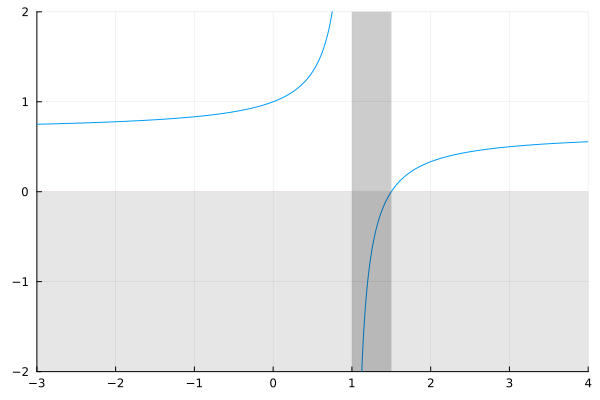
\includegraphics[width=0.5\columnwidth]{./images/wec.png}
\caption{}
\label{}
\end{figure}

\item{$0 \leq \rho(r)$ and $0 \leq \rho(r) + 3p(r)$より}
\begin{equation*}
\begin{split}
	0 \leq & 1 + \frac{ 3p(r) }{ \rho(r) }\\
	\leq & 1 + \frac{ f(r) }{ 1 - f(r) }\\
\end{split}
\end{equation*}
\begin{figure}[H]
\centering
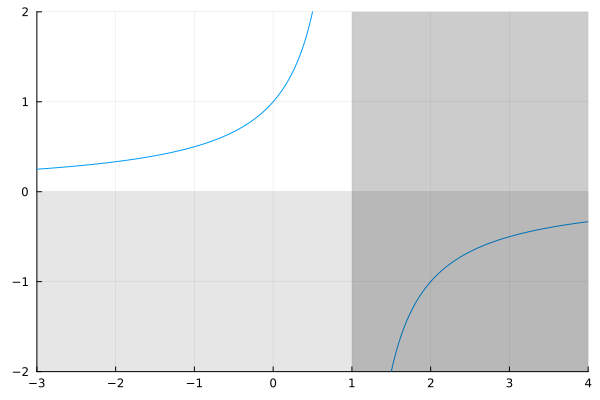
\includegraphics[width=0.5\columnwidth]{./images/sec.png}
\caption{}
\label{}
\end{figure}

\item{$0 \leq \rho(r)$ and $0 \leq \rho(r) - |p(r)|$より}
\begin{equation*}
\begin{split}
	-1 \leq & \frac{ p(r) }{ \rho(r) } \leq 1\\
	-1 \leq & \frac{ f(r) }{ 3 (1 - f(r) ) } \leq 1\\
\end{split}
\end{equation*}
\begin{figure}[H]
\centering
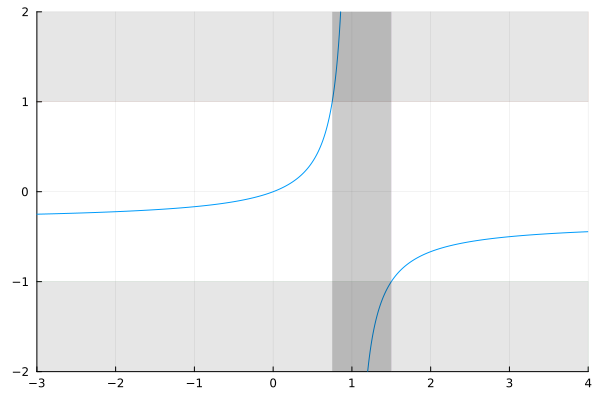
\includegraphics[width=0.5\columnwidth]{./images/dec.png}
\caption{}
\label{}
\end{figure}
\end{enumerate}
以上をまとめると
\[f(r) \leq \frac{3}{4}\]

\subsection{$a$の条件}
上記2つの制約をまとめると
\begin{enumerate}[(1)\,]
\item{$a>0$ and $k>0$ and $f(r) \leq \frac{3}{4}$では}\\
\[0 < a \leq \frac{3}{2}\]
\item{$a>0$ \text{and} $k<0$ここが良くわからない}
\item{$a<0$ \text{and} $k>0$ここが良くわからない}
\item{$a<0$ \text{and} $k<0$ここが良くわからない}
\end{enumerate}

% =================================
% =================================
% =================================
% =================================
% =================================
% Buchdahl
% =================================
% =================================
% =================================
% =================================
% =================================
\chapter{08/01/2025}
\section{Buchdahl時空の曲率}
\begin{equation*}
	g_{ab} = 
	\begin{pmatrix}
   	- \frac{(1 - f(r))^2}{(1 + f(r))^2} & & &\\
   	& (1 + f(r))^4 & &\\
	& & r^2(1 + f(r))^4 &\\
	& & & r^2 (1 + f(r))^4 \sin^2{\theta}\\
	\end{pmatrix}
\end{equation*}
\begin{equation*}
\begin{split}
	f(r) &= \frac{a}{2 \sqrt{1 + kr^2} }\\
	\frac{df}{dr} &= - \frac{ar}{2(1 + kr^2)^{\frac{3}{2}}} = - \frac{af(r)}{1 + kr^2}
\end{split}
\end{equation*}
\[
\tensor{R}{^a_{bcd}} =
	\frac{\partial \tensor{\Gamma}{^a_{bd}}}{\partial x^c}
 	- \frac{\partial \tensor{\Gamma}{^a_{bc}}}{\partial x^d}
	+ \tensor{\Gamma}{^a_{ec}}\tensor{\Gamma}{^e_{bd}}
	- \tensor{\Gamma}{^a_{ed}}\tensor{\Gamma}{^a_{bc}}
\]
\begin{equation*}
\begin{split}
	\frac{g_{tt}}{\partial r} &=
		- \frac{a f(r)}{1 + kr^2} \cdot \frac{2(1 - f(r))}{(1 + f(r))^2}
		- \frac{a f(r)}{1 + kr^2} \cdot \frac{2(1 - f(r))^2}{(1 + f(r))^3}\\
	\frac{g_{rr}}{\partial r} &=
		- \frac{a f(r)}{1 + kr^2} \cdot 4(1 + f(r))^3\\
	\frac{g_{\theta \theta}}{\partial r} &=
		2r(1 + f(r))^4
		- \frac{a f(r)}{1 + kr^2} \cdot 4 r^2 (1 + f(r))^3\\
	\frac{g_{\phi \phi}}{\partial r} &=
		2r(1 + f(r))^4\sin^2\theta
		- \frac{a f(r)}{1 + kr^2} \cdot 4 r^2 (1 + f(r))^3\sin^2\theta\\
	\frac{g_{\phi \phi}}{\partial \theta} &=
		2r^2(1 + f(r))^4\sin\theta\\
\end{split}
\end{equation*}
\subsection{クリストッフェル記号の計算}
\[
\tensor{\Gamma}{^a_{bc}} =
	\frac{1}{2}g^{ad}\left( \frac{\partial g_{db}}{\partial x^c}
	+ \frac{\partial g_{dc}}{\partial x^b}
	- \frac{\partial g_{bc}}{\partial x^d} \right)
\]
クリストッフェル記号がゼロにならない添字の組み合わせ求める。
\begin{enumerate}[(1)\,]
\item{$t=a=d$では}
\begin{equation*}
\begin{split}
	\tensor{\Gamma}{^t_{tr}} = \tensor{\Gamma}{^t_{rt}}
\end{split}
\end{equation*}
\item{$r=a=d$では}
\begin{equation*}
\begin{split}
	\tensor{\Gamma}{^r_{rr}}, \tensor{\Gamma}{^r_{tt}},
	\tensor{\Gamma}{^r_{\theta\theta}}, \tensor{\Gamma}{^r_{\phi\phi}}\\
\end{split}
\end{equation*}
\item{$\theta=a=d$では}
\begin{equation*}
\begin{split}
	&\tensor{\Gamma}{^\theta_{\theta r}} = \tensor{\Gamma}{^\theta_{r \theta}}\\
	&\tensor{\Gamma}{^\theta_{\phi \phi}}
\end{split}
\end{equation*}
\item{$\phi=a=d$では}
\begin{equation*}
\begin{split}
	&\tensor{\Gamma}{^\phi_{\phi r}} = \tensor{\Gamma}{^\phi_{r \phi}}\\
	&\tensor{\Gamma}{^\phi_{\phi \theta}} = \tensor{\Gamma}{^\phi_{\theta \phi}}
\end{split}
\end{equation*}
\end{enumerate}
以上の成分をそれぞれ計算すると
\begin{equation*}
\begin{split}
	\tensor{\Gamma}{^t_{tr}}
		&= \frac{1}{2}(g_{tt})^{-1}\frac{\partial g_{tt}}{\partial r}\\
	\tensor{\Gamma}{^r_{rr}}
		&= \frac{1}{2}(g_{rr})^{-1}\frac{\partial g_{rr}}{\partial r}\\
	\tensor{\Gamma}{^r_{tt}}
		&= - \frac{1}{2}(g_{rr})^{-1}\frac{\partial g_{tt}}{\partial r}\\
	\tensor{\Gamma}{^r_{\theta\theta}}
		&= - \frac{1}{2}(g_{rr})^{-1}\frac{\partial g_{\theta\theta}}{\partial r}\\
	\tensor{\Gamma}{^r_{\phi\phi}}
		&= - \frac{1}{2}(g_{rr})^{-1}\frac{\partial g_{\phi\phi}}{\partial r}\\
	\tensor{\Gamma}{^\theta_{\theta r}}
		&= \frac{1}{2}(g_{\theta\theta})^{-1}\frac{\partial g_{rr}}{\partial \theta}\\
	\tensor{\Gamma}{^\theta_{\phi \phi}}
		&= - \frac{1}{2}(g_{\theta\theta})^{-1}\frac{\partial g_{\phi\phi}}{\partial \theta}\\
	\tensor{\Gamma}{^\phi_{\phi r}}
		&= \frac{1}{2}(g_{\phi\phi})^{-1}\frac{\partial g_{\phi\phi}}{\partial r}\\
	\tensor{\Gamma}{^\phi_{\phi \theta}}
		&= \frac{1}{2}(g_{\phi\phi})^{-1}\frac{\partial g_{\phi\phi}}{\partial \theta}\\
\end{split}
\end{equation*}


/////////////////////////////////////////////////////////////////////////\\
/////////////////////////////////////////////////////////////////////////
\newpage
\noindent

% 行列
\begin{equation*}
\begin{pmatrix}
   a & b \\
   c & d
\end{pmatrix}
\end{equation*}

% 方程式
\begin{equation*}
\begin{split}
	\bar{w}_j = \left( \right) \int^{}_{}
\end{split}
\end{equation*}

% ボックス
\begin{tcolorbox}[title=メモ用]
\begin{eqnarray*}
	1 = 0
\end{eqnarray*}
\end{tcolorbox}

% { 付き方程式
\begin{equation}
\left\{ \,
\begin{aligned}
	1 &= 0\\
	1 &= 0\\
\end{aligned}
\right.
\end{equation}

% 画像
% \begin{figure}[H]
%    \centering
%     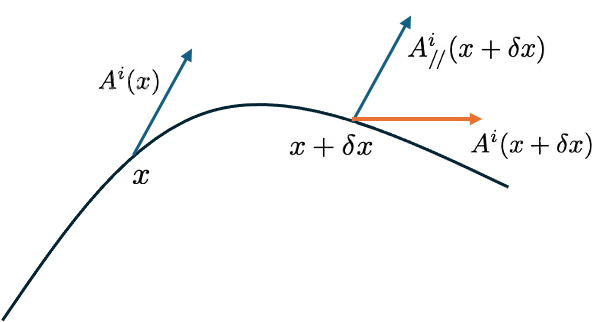
\includegraphics[width=0.5\columnwidth]{./images/0106/01.png}
%     \caption{並行移動}
%     \label{}
% \end{figure}

% リスト
\begin{enumerate}[(1)\,]
\item{}
\end{enumerate}

\end{document}